\documentclass[12pt,]{article}
\usepackage{lmodern}
\usepackage{amssymb,amsmath}
\usepackage{ifxetex,ifluatex}
\usepackage{fixltx2e} % provides \textsubscript
\ifnum 0\ifxetex 1\fi\ifluatex 1\fi=0 % if pdftex
  \usepackage[T1]{fontenc}
  \usepackage[utf8]{inputenc}
\else % if luatex or xelatex
  \ifxetex
    \usepackage{mathspec}
    \usepackage{xltxtra,xunicode}
  \else
    \usepackage{fontspec}
  \fi
  \defaultfontfeatures{Mapping=tex-text,Scale=MatchLowercase}
  \newcommand{\euro}{€}
\fi
% use upquote if available, for straight quotes in verbatim environments
\IfFileExists{upquote.sty}{\usepackage{upquote}}{}
% use microtype if available
\IfFileExists{microtype.sty}{%
\usepackage{microtype}
\UseMicrotypeSet[protrusion]{basicmath} % disable protrusion for tt fonts
}{}
\usepackage[margin=1in]{geometry}
\usepackage{longtable,booktabs}
\usepackage{graphicx}
\makeatletter
\def\maxwidth{\ifdim\Gin@nat@width>\linewidth\linewidth\else\Gin@nat@width\fi}
\def\maxheight{\ifdim\Gin@nat@height>\textheight\textheight\else\Gin@nat@height\fi}
\makeatother
% Scale images if necessary, so that they will not overflow the page
% margins by default, and it is still possible to overwrite the defaults
% using explicit options in \includegraphics[width, height, ...]{}
\setkeys{Gin}{width=\maxwidth,height=\maxheight,keepaspectratio}
\ifxetex
  \usepackage[setpagesize=false, % page size defined by xetex
              unicode=false, % unicode breaks when used with xetex
              xetex]{hyperref}
\else
  \usepackage[unicode=true]{hyperref}
\fi
\hypersetup{breaklinks=true,
            bookmarks=true,
            pdfauthor={Kyle MacDonald; Todd LeMarr; David Corina; Virginia Marchman; Anne Fernald},
            pdftitle={Age-related changes in children's real-time American Sign Language comprehension},
            colorlinks=true,
            citecolor=blue,
            urlcolor=blue,
            linkcolor=magenta,
            pdfborder={0 0 0}}
\urlstyle{same}  % don't use monospace font for urls
\setlength{\parindent}{0pt}
\setlength{\parskip}{6pt plus 2pt minus 1pt}
\setlength{\emergencystretch}{3em}  % prevent overfull lines
\setcounter{secnumdepth}{0}

%%% Use protect on footnotes to avoid problems with footnotes in titles
\let\rmarkdownfootnote\footnote%
\def\footnote{\protect\rmarkdownfootnote}

%%% Change title format to be more compact
\usepackage{titling}

% Create subtitle command for use in maketitle
\newcommand{\subtitle}[1]{
  \posttitle{
    \begin{center}\large#1\end{center}
    }
}

\setlength{\droptitle}{-2em}
  \title{Age-related changes in children's real-time American Sign Language
comprehension}
  \pretitle{\vspace{\droptitle}\centering\huge}
  \posttitle{\par}
  \author{Kyle MacDonald \\ Todd LeMarr \\ David Corina \\ Virginia Marchman \\ Anne Fernald}
  \preauthor{\centering\large\emph}
  \postauthor{\par}
  \date{}
  \predate{}\postdate{}



\begin{document}

\maketitle

\begin{abstract}
Extensive research with children learning spoken language shows that the
ability to interpret speech in real time with high efficiency is
critical to language development (Fernald \& Marchman, 2012). But no
studies have investigated real time language comprehension in young
children learning American Sign Language (ASL). ASL is expressed with
the hands, arms and face, and comprehended with the eyes, differences
that could have potential consequences for how linguistic information is
processed. This cross-sectional study develops the first measures of
ASL-learners' real-time language comprehension skills, and explores
links between these skills and children's vocabulary development. 29
native ASL-learners (16-53 mos) and 19 fluent adult signers completed
measures of language processing efficiency. Children's ASL processing
skills improved with age, and adult signers were more efficient than
children. Importantly, children's processing skills strongly correlated
with their vocabulary size, providing evidence that the ability to
efficiently establish reference in real time is linked to meaningful
linguistic outcomes. These novel findings show that visual language
learners, like children learning spoken languages, make impressive gains
in the efficiency of language interpretation over the first few years of
life as they progress towards adult-like levels of fluency.
\end{abstract}

\newpage

\section{Introduction}\label{introduction}

Understanding language rapidly and accurately is central to our ability
to function effectively in daily life. One fundamental component of
language understanding is linking abstract symbols (i.e.~words and
signs) to concrete objects in the world (i.e., etablishing
reference).\footnote{This problem is also known as the problem of
  referential uncertainty (Quine, 1960): that a speaker's utterance
  could refer to many possible objects in the visual scene, to parts of
  of those objects, or even to something that is not present.} While
children learning spoken languages can simultaneously look at objects
and listen to their caregivers, children learning American Sign Language
(ASL) must rely on vision to both look at objects and to process
linguistic information. This dual functionality requires children to
disengage from the source of language to seek out the named object,
increasing the likelihood of a mapping error or possibly creating a
situation where subsequent information is missed. Thus it is critical to
understand how young ASL-learners establish reference during fluent,
real-time language understanding. In the current work, we aim to develop
the first measures of young ASL-learners' real-time language
comprehension skills, and explore links between these skills and
children's linguistic outcomes.

\subsubsection{Studies of spoken language
comprehension}\label{studies-of-spoken-language-comprehension}

To follow a typical conversation, skilled listeners must rapidly
apprehend meaning in combinations of words from moment to moment as the
speech signal unfolds at rates of 10-15 phonemes/second. Extensive
research with adults using online measures\footnote{Here online measures
  refer to measuring participants' eye movements during language
  comprehension in order to provide a rapid and detailed metric for
  determining the target of their visual attention.} shows that skilled
listeners can identify spoken words before their acoustic offset,
evaluating hypotheses about word identity incrementally based on what
they have heard up to that moment, typically within 150 ms of word onset
(Marslen-Wilson \& Zwitserlood, 1989). Moreover, adults are adept in the
parallel processing of multiple streams of information, rapidly
integrating the acoustic speech signal as it unfolds in time with
information from the visual scene to derive intended meaning (Dahan \&
Tanenhaus, 2004; Tanenhaus et al., 1995; Altmann \& Kamide, 1999, 2004).

Over the past fifteen years, research with infants and young children
has incorporated the same high-resolution measures of language
processing (Fernald, Pinto, Swingley, Weinbergy, \& McRoberts, 1998;
Snedeker \& Trueswell, 2004), making it possible to obtain continuous
measures of speed and accuracy that enable sensitive assessment of
efficiency in spoken language processing even by very young children.
Using these procedures, researchers have found systematic age-related
changes in the speed and accuracy of responses to familiar words
(Fernald et al., 1998), and that efficiency in word recognition is
correlated with both individual differences in vocabulary knowledge
(Fernald, Swingley, \& Pinto, 2001; Zangl, Klarman, Thal, Fernald, \&
Bates, 2005) as well as faster rates of vocabulary growth across the
second year (Fernald, Perfors, \& Marchman, 2006). While studies have
also found associations between faster word recognition and more
advanced linguistic development in both English (Fernald et al., 2001;
Zangl \& Fernald, 2007) and Spanish (Hurtado, Marchman, \& Fernald,
2008; Lew-Williams \& Fernald, 2007), this is the first study to adapt
these online processing efficiency measures to be used with children
learning ASL.

\subsubsection{Psycholinguistics of ASL
comprehension}\label{psycholinguistics-of-asl-comprehension}

ASL is a visual-gestural language expressed with hands, arms and face, a
modality difference with substantial consequences for how linguistic
information is processed. A central question in psycholinguistic studies
of sign language processing with adults has been which aspects of
processing are universal across spoken and signed languages and which
are modality-dependent. In many ways, language processing appears to be
parallel in spoken and manual modalities. Signers show effects of: (a)
lexicality, response times to identify non-signs are slower than for
actual signs (Corina \& Emmorey, 1993), (b) frequency, high frequency
signs are recognized faster than low frequency signs (Carreiras et al.,
2008), and (c) phonological parameters, the sublexical units of sign --
handshape, location, and movement -- influence sign recognition (Corina
\& Emmorey, 1993; Corina \& Hildebrant, 2002; Carreiras et. al., 2008).

However, differences in linguistic structure and surface features of
lexical forms in the spoken vs.~manual modality have consequences for
the efficiency with which signs are understood (Carreiras, 2010, Corina
\& Knapp, 2006). Using a gating procedure, Emmorey and Corina (1990)
found that deaf participants identified monomorphemic signs after
approximately 35\% of the sign form had been seen; in contrast, in
spoken English approximately 83\% of a word must be heard before words
are uniquely identified (Grosjean, 1980). Thus, there is strong evidence
that signs, like spoken words, are processed incrementally by adults,
but we know very little about how young ASL-learners process signs in
real-time.

In sum, this study will be the first to explore the early development of
real-time processing of signs by very young children learning ASL.
First, we adapt a well established paradigm for measuring spoken
language procesing efficiency to be used with young children learning
ASL. Next, we ask whether the development of early ASL comprehension
follows a similar developmental trajectory as that of spoken language.
Finally, we test whether individual variation in ASL processing skills
show similar concurrent relations to children's vocabulary size.

\section{Method}\label{method}

\subsubsection{Participants}\label{participants}

16 deaf and 13 hearing children with native exposure to ASL (17 females,
12 males, Mage = 28.5, range = 16-53months) and 19 fluent adults were
recruited from several locations by bicultural/bilingual researchers
fluent in ASL. All children were exposed to ASL at birth from at least
one fluent ASL caregiver and currently used ASL as their primary mode of
communication at home. The majority of children attended a center-based
early childhood education program in which ASL was the primary mode of
instruction. Thus, children were immersed in ASL early in life, both at
home and in the daycare setting. An additional 20 participants were
tested, but not included in the analyses due to fussiness (n = 5), being
too far outside the target age range (n = 3), and not receiving enough
ASL exposure (n = 12). For visualization purposes, children were divided
into two groups using a median split by age: Younger (\textless{} 26.5
Months), Older (\textgreater{} 26.5 Months), but we conducted all
analyses on individual-level data.

\begin{longtable}[c]{@{}lrrrrrrrr@{}}
\caption{Participant background information. All children were exposed
to ASL from one caregiver from birth.}\tabularnewline
\toprule
Age Group & n & Mean age & Min age & Max age & Female & Male & Deaf &
Hearing\tabularnewline
\midrule
\endfirsthead
\toprule
Age Group & n & Mean age & Min age & Max age & Female & Male & Deaf &
Hearing\tabularnewline
\midrule
\endhead
\textless{} 26.5 Months & 14 & 20.8 & 16 & 26 & 8 & 6 & 7 &
7\tabularnewline
\textgreater{} 26.5 Months & 15 & 35.7 & 27 & 53 & 9 & 6 & 9 &
6\tabularnewline
\bottomrule
\end{longtable}

\subsubsection{Measures}\label{measures}

\emph{Parent report of vocabulary size}: Parents completed a 90-item
vocabulary checklist designed to be culturally and linguistically
appropriate for children learning ASL. Vocabulary size was computed as
the number of reported signs produced.

\emph{ASL Processing}: Efficiency in online comprehension was assessed
using a version of the looking-while-listening procedure (LWL) (Fernald
et al., 2006; Fernald, Zangl, Portillo \& Marchman, 2008) adapted for
ASL-learners, which we call the Visual Language Processing (VLP) task.
Since this was the first study to measure online ASL processing
efficiency in young signers, several critical modifications were made,
which we describe below.

\subsubsection{Apparatus}\label{apparatus}

A portable version of the VLP was created to facilitate recruitment of
participants. Stimuli were presented on a portable 27'' monitor using a
Macbook Pro laptop. Video of the child's eye gaze was recorded using a
digital camcorder set up behind the monitor. To minimize visual
distractions, children sat on their caregivers' laps inside of a
portable 5' by 5' tent with opaque walls.

\begin{figure}[htbp]
\centering
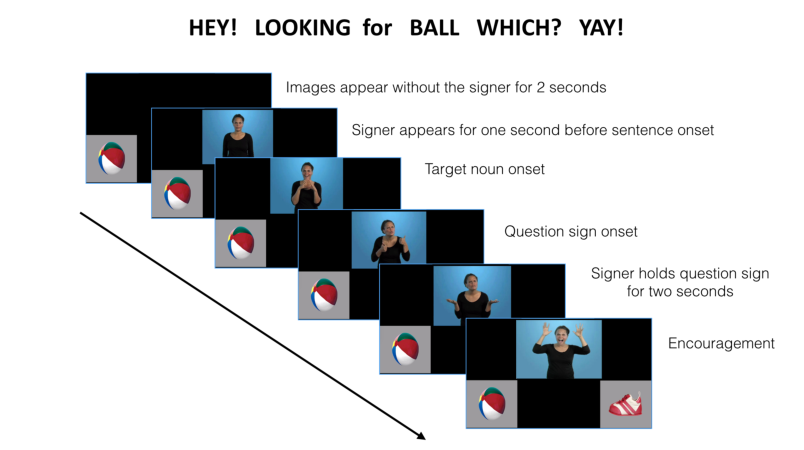
\includegraphics{Figs/timeline-1.pdf}
\caption{Timeline of a trial on the VLP task. On each trial the child
saw two images on the screen for two seconds before the signer appeared.
A one second still frame of the signer gave children the opportunity to
orient to the signer before sentence onset. Each sentence lasted for
approximately five seconds and was followed with a two second ``hold''
that allowed children to shift away from the signer to the images on the
screen. After the hold, the signer gave neutral, positive feedback to
help maintain the child's focus throughout the task.}
\end{figure}

\subsubsection{Trial Structure}\label{trial-structure}

On each trial, children saw pictures of two familiar objects and a
signer naming one of them. Figure 1 shows an example of the stimuli and
the timeline of one trial in the VLP task. Each trial lasted
approximately 7-8 secs.

\subsubsection{Linguistic and visual
stimuli}\label{linguistic-and-visual-stimuli}

The linguistic stimuli were designed to be comparable to those used in
previous research and to allow for generalization beyond characteristics
of a specific signer and sentence structure. To accomplish this, ASL
stimuli were recorded by two different native ASL-users using two
different but acceptable ASL sentence structures for asking
questions\footnote{See Neidle, Kegl, Bahan, Aarons, \& MacLaughlin
  (1997) for a detailed discussion of the acceptability of these two
  question structures.}:

\begin{itemize}
\itemsep1pt\parskip0pt\parsep0pt
\item
  Sentence-initial wh-phrase: ``HEY! WHERE {[}target noun{]}?''
\item
  Sentence-final wh-phrase: ``HEY! {[}target noun{]} WHERE?''
\end{itemize}

Before each sentence, the signer used a hand-waving gesture commonly
used in ASL discourse to get the child's attention.

Four yoked pairs of eight target nouns (cat---bird, car---book,
bear---doll, ball---shoe) were used. These nouns were selected such that
they would be familiar to most children learning ASL at this age and
have minimal phonological overlap. To prepare the stimuli, a female
native ASL-user recorded several tokens of each sentence, matching them
closely in prosody. These candidate stimuli were then digitized,
analyzed, and edited using Final Cut Pro software. The final tokens were
chosen based on naturalness and prosodic comparability. The mean
duration of target nouns was TODO ms (range = TODO ms). Five filler
trials were interspersed among the 32 test trials (e.g. ``YOU LIKE
PICTURES! MORE WANT?''). Images were digitized pictures presented in
fixed pairs, matched for visual salience with 3--4 tokens of each object
type. Side of target picture was counterbalanced across trials.

\subsubsection{Coding and reliability}\label{coding-and-reliability}

Children's gaze patterns were videotaped and coded frame-by-frame,
yielding a high-resolution record of eye movements aligned with target
noun onset. 25\% of videos were re-coded to assess coder reliability --
agreement within a single frame averaged 98\% on these reliability
assessments.

\subsubsection{Calculating linguistic processing
efficiency}\label{calculating-linguistic-processing-efficiency}

Correct looking is a function of the child's tendency to shift quickly
away from the central signer to the target picture in response to the
target sign, and also to remain fixated on the target picture. To
determine the degree to which participants fixated the appropriate
picture across trials, mean proportion looking to target was calculated
for each participant at each 33 ms frame from the onset of the target
noun. Accuracy was defined as the mean proportion of time spent looking
at the target picture out of the total time spent on either the target
picture, the distracter picture, or the signer from 500 to 2000 ms from
target noun onset. Importantly, the VLP task includes a central signer,
which functions as a central fixation point similar to adult
psycholinguistic experiments. Thus children could produce four different
types of responses on a given trial: (1) signer-to-target shift, (2)
signer-to-distractor shift, (3) signer-to-away shift, (4) no-shift. All
four trial types contribute to accuracy analyses.

Reaction time (RT) corresponds to the latency to shift away from the
signer to the target picture, measured from the onset of the target
sign. Responses prior to 500 ms from noun onset were excluded because
very few responses occurred before this cut point, presumably because
the child did not have enough time to process sufficient linguistic
input and to mobilize an eye movement; responses slower than 2000 ms
were excluded because these delayed looks are less likely to reflect a
response to the target sign (see Fernald, Swingley \& Pinto, 2001). This
window was selected such that 90\% of all trials with a signer-to-target
shift were included in the analysis. In addition, 8\% of trials were
excluded because children never shifted off the signer. Note that RT can
be calculated only on those trials on which the child is looking at the
signer at the onset of the noun and shifts within the designated time
window. Since children vary in the likelihood that they will shift on a
given trial, mean RTs are based on different numbers of trials across
participants (M=13.4 trials, range=3---25). All children had at least
three RTs within the appropriate window and were included in the
analyses.

\subsubsection{Bayesian data analysis}\label{bayesian-data-analysis}

TODO: explain why we chose to use latent mixture model

\section{Results}\label{results}

First we present analyses of performance on the VLP task, showing that
children become faster and more accurate at comprehending familiar signs
as they get older and progress towards adult levels of language fluency.
Then we present an analysis of the links between children's real time
ASL processing skills and productive ASL vocabulary.

\begin{figure}[htbp]
\centering
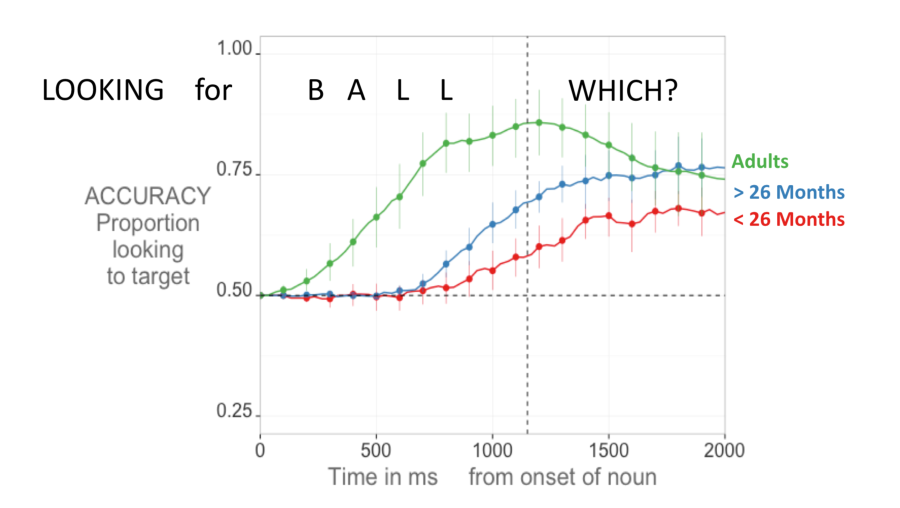
\includegraphics{Figs/profile plot png-1.pdf}
\caption{The accuracy of participants' looking to target picture as a
function of age group (Younger children, Older children, and Adults).
Curves show changes over time in the mean proportion looking to the
correct picture, measured in ms from noun onset; error bars represent
+/- 95\% CI computed by non-parametric bootstrap. The dashed vertical
line indicates mean offset of target noun (TODO ms). Mean accuracy
scores were computed over a window from 500--2000 ms from noun onset.}
\end{figure}

\subsubsection{ASL processing
efficiency}\label{asl-processing-efficiency}

Figure 3 provides an overview of the time course of correct orienting to
the referent in response to the target sign. The three curves show
changes in the mean proportion of trials on which participants in each
age group fixated the correct referent at every 33 ms interval as the
target sign unfolded. Before seeing the target sign, all participants
fixated on the signer. Both adults and children began to increase their
looking to the target picture before the offset of the target noun. But
children remained at chance for approximately 700 milliseconds longer
than adults, with the youngest children taking the longest to look to
the target over the trial. Differences in asymptote reflect the higher
levels of accuracy achieved by older children and the adults.

\emph{Accuracy:} Mean accuracy scores, computed over the 500--2000 ms
window from noun onset, were examined as a function of age. Accuracy was
strongly correlated with age (r(27) = 0.64), indicating that older
ASL-learners were significantly more reliable than younger children in
fixating the target picture.

\emph{Reaction Time:} Mean reaction times were negatively correlated
with age (r(22) = -0.38), indicating that older ASL-learning children
were faster to shift to the target picture than younger ones. Mean
reaction times were also negatively correlated with mean accuracy scores
(r(22) = -0.59) such that those children who were faster to shift to the
target were also more likely to stick on the target image thoughout the
analysis window.

\subsubsection{Links between processing efficiency and ASL
vocabulary}\label{links-between-processing-efficiency-and-asl-vocabulary}

\begin{figure}[htbp]
\centering
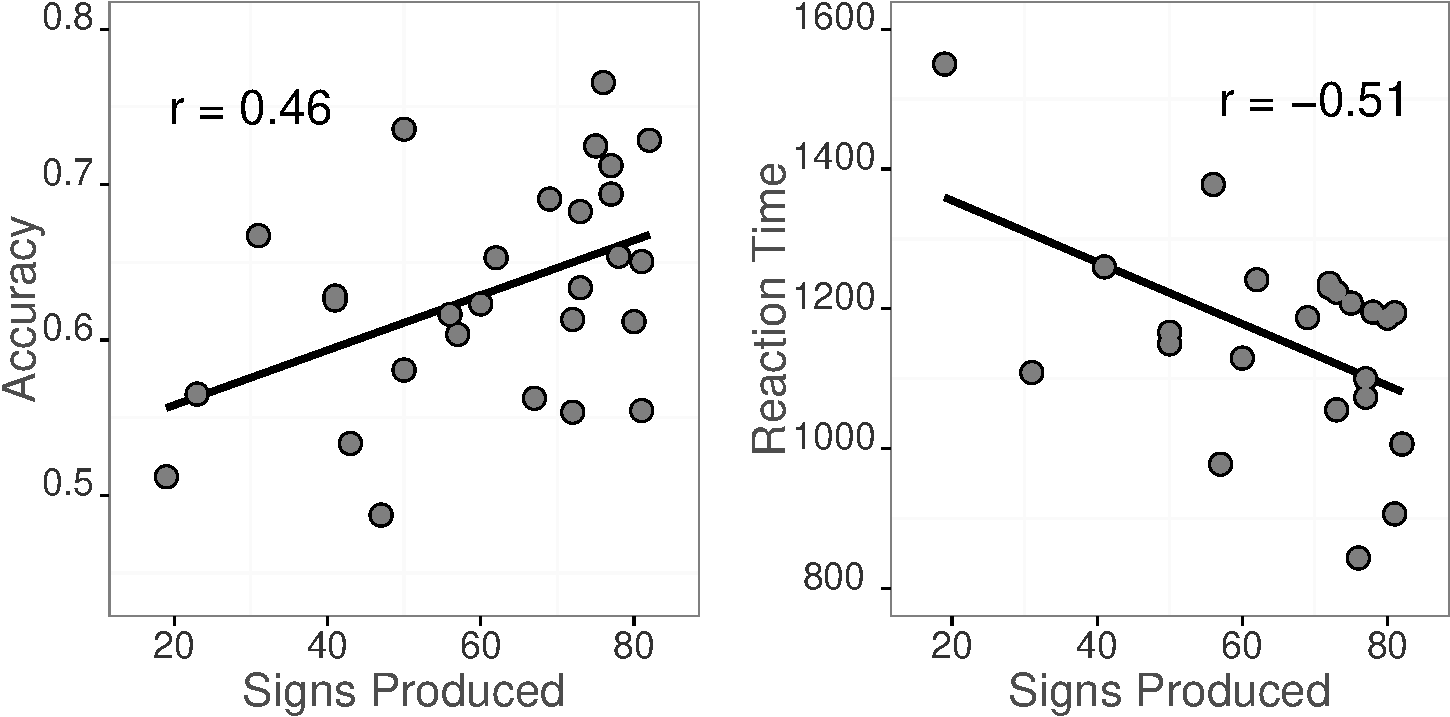
\includegraphics{Figs/vocab scatter plots-1.pdf}
\caption{Relationship between VLP measures and productive ASL
vocabulary. Each data point is an individual child. Panel A shows the
positive relationship between accuracy and vocabulary. Panel B shows the
negative relationship between RT and vocabulary}
\end{figure}

Figure 4 shows the relationships between both VLP processing measures
and children's productive ASL vocabulary. Mean accuracy was positively
related to vocabulary size (r(26) = 0.46) such that children with higher
accuracy scores also had larger productive vocabularies. Mean reaction
times were negatively correlated with vocabulary (r(21) = -0.51)
indicating that children who were faster to recognize ASL signs also had
larger vocabularies.

It is important to point out that age and vocabulary were strongly
intercorrelated in our sample (r(21) = 0.72). In a multiple regression
analysis\ldots{} (TODO: figure out how to talk about regression
analysis)

\section{Discussion}\label{discussion}

\newpage 

\section*{References}\label{references}
\addcontentsline{toc}{section}{References}

Fernald, A., \& Marchman, V. A. (2012). Individual differences in
lexical processing at 18 months predict vocabulary growth in typically
developing and late-talking toddlers. \emph{Child Development},
\emph{83}(1), 203--222.

Fernald, A., Perfors, A., \& Marchman, V. A. (2006). Picking up speed in
understanding: Speech processing efficiency and vocabulary growth across
the 2nd year. \emph{Developmental Psychology}, \emph{42}(1), 98.

Fernald, A., Pinto, J. P., Swingley, D., Weinbergy, A., \& McRoberts, G.
W. (1998). Rapid gains in speed of verbal processing by infants in the
2nd year. \emph{Psychological Science}, \emph{9}(3), 228--231.

Fernald, A., Swingley, D., \& Pinto, J. P. (2001). When half a word is
enough: Infants can recognize spoken words using partial phonetic
information. \emph{Child Development}, \emph{72}(4), 1003--1015.

Hurtado, N., Marchman, V. A., \& Fernald, A. (2008). Does input
influence uptake? Links between maternal talk, processing speed and
vocabulary size in spanish-learning children. \emph{Developmental
Science}, \emph{11}(6), F31--F39.

Lew-Williams, C., \& Fernald, A. (2007). Young children learning spanish
make rapid use of grammatical gender in spoken word recognition.
\emph{Psychological Science}, \emph{18}(3), 193--198.

Marslen-Wilson, W., \& Zwitserlood, P. (1989). Accessing spoken words:
The importance of word onsets. \emph{Journal of Experimental Psychology:
Human Perception and Performance}, \emph{15}(3), 576.

Quine, W. (1960). \emph{Word and object}. MIT press.

Snedeker, J., \& Trueswell, J. C. (2004). The developing constraints on
parsing decisions: The role of lexical-biases and referential scenes in
child and adult sentence processing. \emph{Cognitive Psychology},
\emph{49}(3), 238--299.

Zangl, R., \& Fernald, A. (2007). Increasing flexibility in children's
online processing of grammatical and nonce determiners in fluent speech.
\emph{Language Learning and Development}, \emph{3}(3), 199--231.

Zangl, R., Klarman, L., Thal, D., Fernald, A., \& Bates, E. (2005).
Dynamics of word comprehension in infancy: Developments in timing,
accuracy, and resistance to acoustic degradation. \emph{Journal of
Cognition and Development}, \emph{6}(2), 179--208.

\end{document}
